\documentclass{dsekprotokoll}

\usepackage[T1]{fontenc}
\usepackage[utf8]{inputenc}
\usepackage[swedish]{babel}
\usepackage{tikz}
\usetikzlibrary{arrows.meta,positioning}

\setheader{Policy för Ekonomi}{Policydokument}{}

\title{Policy för ekonomi}
\author{D-sektionen}

\begin{document}
\maketitle
\section{Formalia}
\subsection{Sammanfattning}
Policyn beskriver hur sektionen ska arbeta med ekonomi och budget, hur
attesteringsrätten fungerar samt vilka fonder sektionen har.

\subsection{Syfte}
Policyns syfte är att ge styrelsen såväl som funktionärer vägledning i
ekonomiska frågor.

\subsection{Omfattning}
Sektionen i sin helhet.

\subsection{Historik}
Ursprungligen antagen enligt beslut: VTM 2017.
Omarbetning fastställd enligt beslut (samt motionär):
\begin{itemize}
\item VTM 2021 (Joel Bäcker \& Sean Jentz)
\item (uppdaterad enl. Policy för Policyer på HTM2 2021)
\item VTM 2022 (Emma Kujala)
\item (uppdaterad enl. Policy för styrdokument på HTM2 2021)
\item HTM2 2023 (Axel Svensson)
\end{itemize}

\section{Övergripande}
D-sektionen är en ideell förening och har inget vinstintresse. Därmed skall
ingen funktionär inom D-sektionen behöva betala pengar ur egen ficka för att
kunna utföra sitt uppdrag så som uppdraget är beskrivet i reglementet. Ingen
funktionär ska tjäna pengar på sektionens verksamhet.

\section{Budget}

\subsection{Terminologi}

\begin{description}
  \item[Resultatenhet] Varje utskott, Styrelsen och Sektionen är var och en sin
    egen resultatenhet. Resultatenheten är uppdelad i ett eller flera
    kostnadsställen.
  \item[Kostnadsställe] Ett kostnadsställe består av budgetposter för både
    kostnader och inkomster för en viss del av en resultatenhets
    verksamhet. Varje kostnadsställe har en egen kod, till exempel är SEKT01 ett
    kostnadsställe inom resultatenheten ``sektionen''.
  \item[Budgetpost] En budgetpost visar hur mycket sektionen har budgeterat för
    en viss kostnad eller inkomst. Till exempel är \textit{mötesfika} och
    \textit{programvaror} båda budgetposter.
\end{description}

\subsection{Övergripande}
Sektionsmötet beslutar varje höst om rambudgeten för det kommande året som ett
styrmedel för resultaten i varje kostnadsställe. Likadant beslutar styrelsen
om en detaljbudget under våren för att styra enskilda budgetposters storlek inom
kostnadsställena.

En budget är att betrakta som en prognos för det kommande årets resultat. För
att möjliggöra smidiga anpassningar efter verkligt utfall så krävs ett visst
handlingsutrymme utanför rambudget respektive detaljbudgeten.

\subsection{Budgetavsteg}
Om en budgetpost inom ett kostnadställe, hela kostnadsstället eller rambudgeten
i sin helhet avsiktligt beräknas avvika negativt kan ett budgetavsteg göras.

Summan av de budgetavsteg som tas mellan två stycken redovisningstillfällen
(sektions- och styrelsemöten) får totalt inte överstiga gränsen som kräver
beslut från den högre instansen.  Till exempel så kan inte styrelsen ta två
budgetavsteg à 20 000 kr på ett och samma kostnadsställe utan att först redovisa
det första för sektionsmötet innan det andra tas.  På samma sätt kan inte
skattmästaren ta två budgetavsteg à 1500 kr på samma budgetpost utanatt redovisa
det första för styrelsen först.

\begin{center}
  \renewcommand{\arraystretch}{1.75}
  \begin{tabular}{p{0.2\textwidth}|p{0.4\textwidth}|p{0.3\textwidth}}
    Ekonomiskt objekt & Förändring & Vem ska ta budgetavsteget \\ \hline
    Rambudgeten i sin helhet & Större än 50 000 kr eller mer än 50\% av
    budgeterat resultat & Sektionsmötet \\
    Rambudgeten i sin helhet & Mindre än 50 000 kr och mindre än 50\% av
    budgeterat resultat* & Styrelsen \\
    Kostnadsställe & Större än 25 000 kr eller mer än 50\% av budgeterat
    resultat & Sektionsmötet \\
    Kostnadsställe & Mindre än 25 000 kr och mindre än 50\% av budgeterat
    resultat* & Styrelsen \\
    Budgetpost inom kostnadställen & Budgetavsteg på max 2500 kr & Skattmästaren
    i samråd med sektionsordförande
  \end{tabular}
  \renewcommand{\arraystretch}{1.0}
\end{center}
* --- För rambudget och kostnadsställen kan styrelsen alltid ta budgetavsteg om summor lägre
än 10 000 kr även om detta är mer än 50\% av budgeterat resultat.

Budgetavstegen ska vara skriftliga och dokumenteras för verksamhetens ekonomiska
kontinuitet. När budgetavsteg görs av skattmästaren och sektionsordföranden ska
dessa redovisas på ett styrelsemöte eller som ett per capsulambeslut minst en
gång i månaden eller oftare om skattmästaren anser det vara lämpligt.
Styrelsens och skattmästarens budgetavsteg ska redovisas på nästkommande
sektionsmöte.

\section{Avtal}
Firmatecknare äger alltid rätt att besluta om avtal som innebär ett positivt nettoresultat och om
avtal som följer redan lagd budget. En förutsättning är att avtalet inte går emot sektionens eller
Teknologkårens styrdokument.

\section{Sektionskort}
Sektionen äger ett antal betalkort, ofta kallade Sektionskort, som ska användas för betalning i
sektionens namn. Dessa betalkort skall användas för att minimera behovet av privata utlägg.

Vilka som erhåller sektionskort bestäms av styrelsen.

\section{Inköp för sektionen}
Alla köp i sektionens namn, vare sig privata eller med sektionskort, ska
redogöras för genom en utläggsräkning tillsammans med ett fysiskt
kvitto. Kontoutdrag räknas inte. Utläggsräkningar skall skyndsamt lämnas in till
skattmästeriet om ej särskilda skäl finns.

Samtliga utlägg skall signeras av två individer, personen som gjort utlägget och
en som godkänner utlägget. Godkännandet ska, om möjligt, utföras av individ
från den närmst följande instansen enligt nästa avsnitt. En högre instans
signatur kan i samtliga fall ersätta en lägre instans signatur om så
behövs. En lägre instans kan aldrig godkänna en högre instans utlägg. En individ
signerar alltid i egenskap av sin högsta instans.

Utlägg kan inte godkännas av samma individ som gjort utlägget.

\subsection{Attesträtt}
Nedan följer hur attesteringsrätt fungerar för mästare, vice skattmästare och
firmatecknare.  Attest ska alltid sträva efter att skötas på lägsta möjliga
instans. Diagrammet nedan är endast för vägledning, nedanstående punkter
beskriver mer exakta bestämmelser.

Utskott som inte har en utskottsordförande som inte sitter i styrelsen och
projektgrupper vänder sig till firmatecknare för att få sina utlägg
attesterade.

\begin{description}
  \item[Firmatecknare] äger attesteringsrätt för alla utlägg och kan attesteras
    av varandra. Firmatecknare kan inte attestera sina egna utlägg.
  \item[Vice skattmästare] äger attesteringsrätt för alla utlägg gjorda av
    funktionärer. Vice skattmästare kan inte attestera styrelseledamöter.
  \item[Näringslivsansvarig] äger attesteringsrätt för alla utlägg gjorda för
    näringslivsutskottet, inklusive utlägg gjorda av Teknikfokusansvarig.
  \item[Aktivitetsansvarig] äger attesteringsrätt för alla utlägg gjorda för
    aktivitetsutskottet, inklusive UtEDischoansvarig.
  \item[Övriga styrelseledamöter] äger attersteringsrätt för utskott för vilka
    dem är utskottsordförande. Alltså har Vice Ordförande inte någon
    attesteringsrätt.
  \item[Teknikfokusansvarig] äger attesteringsrätt för alla utlägg gjorda för
    Teknikfokus.
\end{description}

\begin{center}
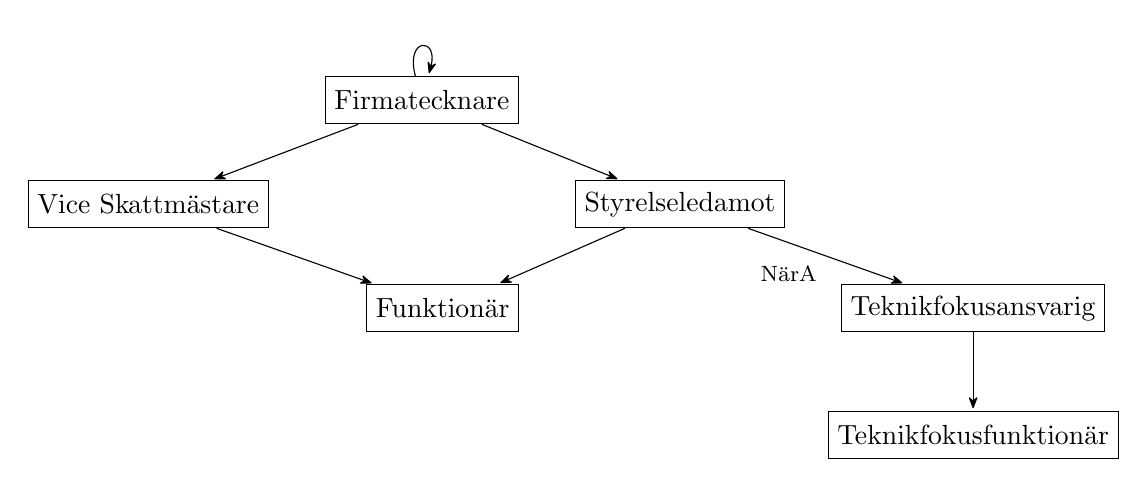
\begin{tikzpicture}
  [shorten >=1pt,
   node distance=1cm,
%% on grid,
   >={Stealth[round]},
   squarednode/.style={rectangle,
                      draw=black,
                      minimum size=6mm},]
  \node[squarednode] (ft)                          {Firmatecknare};
  \node[squarednode] (vice)   [below left=of ft]   {Vice Skattmästare};
  \node[squarednode] (styr)   [below right=of ft]  {Styrelseledamot};
  \node[squarednode] (funk)   [below left=of styr] {Funktionär};
  \node[squarednode] (tekf)   [below right=of styr]{Teknikfokusansvarig};
  \node[squarednode] (tekf-f) [below=of tekf]      {Teknikfokusfunktionär};
  \path[->,every node/.style={font=\footnotesize}]
  (ft)   edge [loop above] node               {} ()
         edge              node [below left]  {} (vice)
         edge              node [below right] {} (styr)
  (vice) edge              node [below right] {} (funk)
  (styr) edge              node [below left]  {} (funk)
         edge              node [below  left] {NärA} (tekf)
  (tekf) edge              node [below]       {} (tekf-f);
\end{tikzpicture}
\end{center}

\section{Kontanthantering}
Sektionen ska eftersträva minimal kontanthantering och istället jobba med
digitala betalningsalternativ.

Kontantbelopp som överstiger 3000 kr skall och måste räknas av minst två
personer.

\section{Likviditet}
Sektionens grundlikviditet bör vara 500 000 kr. Tillfälliga negativa avvikelser
är godtagbara i samband med större arrangemang såsom nollning, jubileum eller
Teknikfokus.

\section{Donationer}

\subsection{Inkomna donationer}
Vid inkomna donationer ska dessa pengar öronmärkas för ett specifik ändamål samt
läggas i lämplig fond. I de fall där inget specifikt ändamål angetts hanteras de
som om det inte fanns en specifik fond och behöver således inte heller
öronmärkas till något speciellt.  Styrelsen kan ta emot och disponera donationer
upp till 10 000 kr men högre än så måste ett sektionsmötesbeslut avgöra hur man
ska disponera pengarna.

\subsection{Utgående donationer}
Vid försäljning av varor kan ett utskott välja att ta emot donationer som ska gå
till olika ickevinst drivande, ideella, välgörenhetsorganisationer. Dessa
pengar ska inte användas av något annat än till dessa ändamål. Styrelsemöte
avgör organisationens lämplighet.

\section{Sektionens fonder}
Sektionen fonderar medel vid bokslutsdispositionen, öronmärkta för att användas
till vissa specifika saker. Nedan följer en lista på sektionens fonder och
vilken instants som disponerar respektive fond följt av en
fondavsättningsstrategi. Vid inköp som inte passar in på någon av fonderna ska
inköpet belasta verksamhetsårets resultat.

Sektionens årliga budget bör avsätta medel till de fonder som behöver det enligt
fondens beskrivning. I händelse av att en fond redan är fylld då pengarna
skall överföras bör de budgeterade pengarna som överskrider maxtaket för
fonden läggas till resultatet. Samtliga uttag ur någon av fonderna skall
redovisas för nästkommande sektionsmöte.

\subsection{Reparationsfonden}
Reparationsfondens syfte är att finansiera ersättande eller reparation av dyra
inventarier (exklusive sektionsbil) som går sönder. Reparationsfonden får
uppgå till maximalt 40 000 kr och dess medel disponeras av styrelsen. Den årliga
budgeten bör avsätta 10 000 kr till fonden årligen.

\subsection{Bilfonden}
Bilfondens medel skall nyttjas till att kunna reparera skador på sektionens bil
samt tillse att den är säker att köra. I händelse av att sektionen behöver
införskaffa en ny bil kan pengarna ur fonden också nyttjas. Fonden får maximalt
uppgå till 60 000 kr och dess medel disponeras av styrelsen. Den årliga budgeten
bör avsätta 10 000 kr till fonden årligen.

\subsection{Projektfonden}
Projektfonden syftar till att kunna avsätta medel för projekt inom
D-sektionen. Dessa projekt skall pågå under en begränsad tid och vara till nytta
för sektionen eller dess medlemmar. Fonden får uppgå till maximalt 20 000 kr
och dess medel disponeras av styrelsen. Den årliga budgeten bör avsätta 5000
kr till fonden årligen.

\subsection{Medaljfonden}
Medaljfonden syftar till att kunna köpa in de medaljer som sektionen, enligt
vårt reglemente, skall delas ut till funktionärer, riddare eller
liknande. Medaljfondens medel kan också nyttjas till framtagande av nya medaljer
som sektionsmötet beslutat om. Fondens medel får maximalt uppgå till 10 000 kr
och de disponeras av styrelsen. Den årliga budgeten bör avsätta 2000 kr till
fonden årligen.

\subsection{Jubileumsfonden}
Jubileumsfonden syftar till att kunna finansiera sektionens jubileumsfirande
vart femte år.  Pengarna skall nyttjas för att säkerställa tillgängligheten för
medlemmarna på jubileumsfirandet. Fondens medel disponeras av styrelsen.
Fondens medel får uppgå till maximalt 50 000 kr.  Den årliga budgeten bör
avsätta 10 000 kr till fonden årligen och bör inte heller överstiga detta om
inte särskilda skäl finnes.

\subsection{Motionsfonden}
Motionsfonden syftar till att kunna genomföra de motioner som föreslås av
medlemmarna till sektionsmötet och som sedan röstas igenom där. Fonden har inget
maxtak på mängden pengar som får finnas i den och dess medel får endast nyttjas
av sektionsmötet.

\subsection{Fondavsättningsstrategi}
Fondavsättningen bör följa denna ordning om inte särkilda fall finnes:
\begin{enumerate}
  \item reparationsfonden,
  \item bilfonden,
  \item projektfonden,
  \item medaljfonden,
  \item jubileumsfonden,
  \item motionsfonden.
\end{enumerate}

\section{Placeringar}
Om sektionen har placeringar bör dessa följa de etiska hänsynstagande som finns
i Teknologkårens policy för ekonomi.

\end{document}
